\documentclass{bmd2010a}

\begin{document}

\begin{flushleft}
{\fontsize{16pt}{20pt}\selectfont%
  Instructions for Preparing an Abstract for the Bicycle and\\}
{\fontsize{16pt}{20pt}\selectfont%
  Motorcycle Dynamics Symposium\\}
\end{flushleft}

%%%%%%%%%%%%%%%% authors %%%%%%%%%%%%%%%
\begin{flushleft}
  {\fontsize{12}{14}{A. B. Author}\\}
  \textit{Faculty of Mechanical Engineering\\
          University of Technology\\
          Address, Postcode City, Country\\
          e-mail: email1@address
}\vspace{10pt}\\
  {\fontsize{12}{14}{C. Author}\\}
  \textit{Affiliation}\vspace{10pt}\\
  {\fontsize{12}{14}{D. E. Author}\\}
  \textit{Affiliation}\vspace{10pt}\\
\end{flushleft}

\section*{Abstract}
Authors are requested to upload an abstract of two pages (including references
and figures) by the stated date in the call for papers to the symposium web
site http://bicycle.tudelft.nl/bmd2010. The uploaded file must use the
Portable Document Format (PDF) and the file should have a sensible name like: Surname1Surname2Surname3\_abstract.pdf.

The abstract must be written in English. It must contain the name, affiliation
and e-mail address of the authors. The header should be as in
this example. The text area is 24 by 15~cm, with left and right margins of
3~cm and a top margin (not including the header) of 3~cm. The paper used should have the size 210 x 297 mm which is the European A4 size. The title should be
in Times New Roman 16pt, and may extend over more than one line. The author's
name or authors' names should be in Times New Roman 12 pt, and the affiliation
should be in 11pt italics.

The abstract itself has the section heading \textbf{Abstract}, bold 11~pt
Times New Roman, and the text should be written in Times New Roman, 11~pt.

Equations should be numbered continuously according to the format
shown in Equation~(\ref{eq:equ1}):
\begin{equation} \label{eq:equ1}
e^{i\pi} + 1 = 0,
\end{equation}
where the unknown symbols are explained after the equation.

\begin{table}[h!]
\begin{center}
\caption{Example of a table with a short caption.} \label{tab:tab1}
\begin{tabular}{|c|ccc|}
\hline
    &  $x$  &  $y$  &  $z$ \\
\hline
$x'$  &  $\alpha_1$ & $\beta_1$ & $\gamma_1$ \\
$y'$  &  $\alpha_2$ & $\beta_2$ & $\gamma_2$ \\
$z'$  &  $\alpha_3$ & $\beta_3$ & $\gamma_3$ \\
\hline
\end{tabular}
\end{center}
\end{table}


Figures, graphs
and tables must be included using the same style as in Figure~\ref{fig:fig1}
and Table~\ref{tab:tab1}. Both figures and tables should be centred on the page. Use of at least 300 dpi resolution for pictures and 600 dpi for line art is required, 1 px wide lines in figures should be avoided as they may become invisible in print.

Bibliographical citations should be written in the
order in which they are cited, see the References section below, where
Reference~\cite{Pac02} exemplifies the case of a textbook, while
Reference~\cite{Ber07} is an article in conference proceedings and
Reference~\cite{Sha71} is an article in a journal. Use can be made of a
pre-existing bibtex style which uses a similar style.


The full paper will have a similar style, but with a different style file. Templates can be found at the symposium website in due time.


\begin{figure}[h!]
\begin{center}
  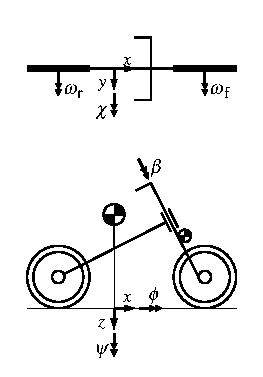
\includegraphics[width=55mm]{figure1}
  \caption{An example of a figure caption. Use 10~pt Times New Roman.
           For long captions, use a text width of 13~cm.
           Use the same style for the tables.} \label{fig:fig1}
\end{center}
\end{figure}


We very much look forward to welcoming you in Delft! Best wishes and the warmest regards from the Organizing Committee of Bicycle and Motorcycle Dynamics 2010.


% \bibliographystyle{acm}
% \bibliography{biblio}
\begin{thebibliography}{6}
% \begin{thebibliography}{66} % use this for more than 9 references
\bibitem{Pac02} H.~B.~Pacejka,
\textit{Tyre and Vehicle Dynamics},
Butterworth and Heinemann, Oxford, 2002.

\bibitem{Ber07} E.~Bertolazzi, F.~Biral, M.~Da~Lio and V.~Cossalter,
``The influence of rider's upper body motions on motorcycle minimum time
  maneuvering'',
in C.~L.~Bottasso, P.~Masarati and L.~Trainelli (eds),
\textit{Proceedings, Multibody Dynamics 2007, ECCOMAS Thematic Conference},
Milano, Italy, 25--28 June 2007,
Politecnico di Milano, Milano, 2007, 15~pp.

\bibitem{Sha71} R.~S.~Sharp,
``The stability and control of motorcycles'',
\textit{Proceedings of the IMechE, Part C, Journal of Mechanical Engineering
  Science} \textbf{13} (1971), pp.~316--329.

\end{thebibliography}

\end{document}
